\normaltrue \difficilefalse \tdifficilefalse
\correctionfalse

%\UPSTIidClasse{11} % 11 sup, 12 spé
%\newcommand{\UPSTIidClasse}{12}

\exer{Calcul de moment$\star$ \label{STAT:02:B2:14-gl:519}}
\setcounter{question}{0}\marginnote{\xpComp{STAT}{02}}%\UPSTIcompetence[2]{B2-14}
\index{Compétence STAT-02}
%\index{La Seine Musicale}
\ifcorrection
\else
\marginnote{\textbf{Pas de corrigé pour cet exercice.}}
\fi

\ifprof
\else


\begin{marginfigure}
\centering
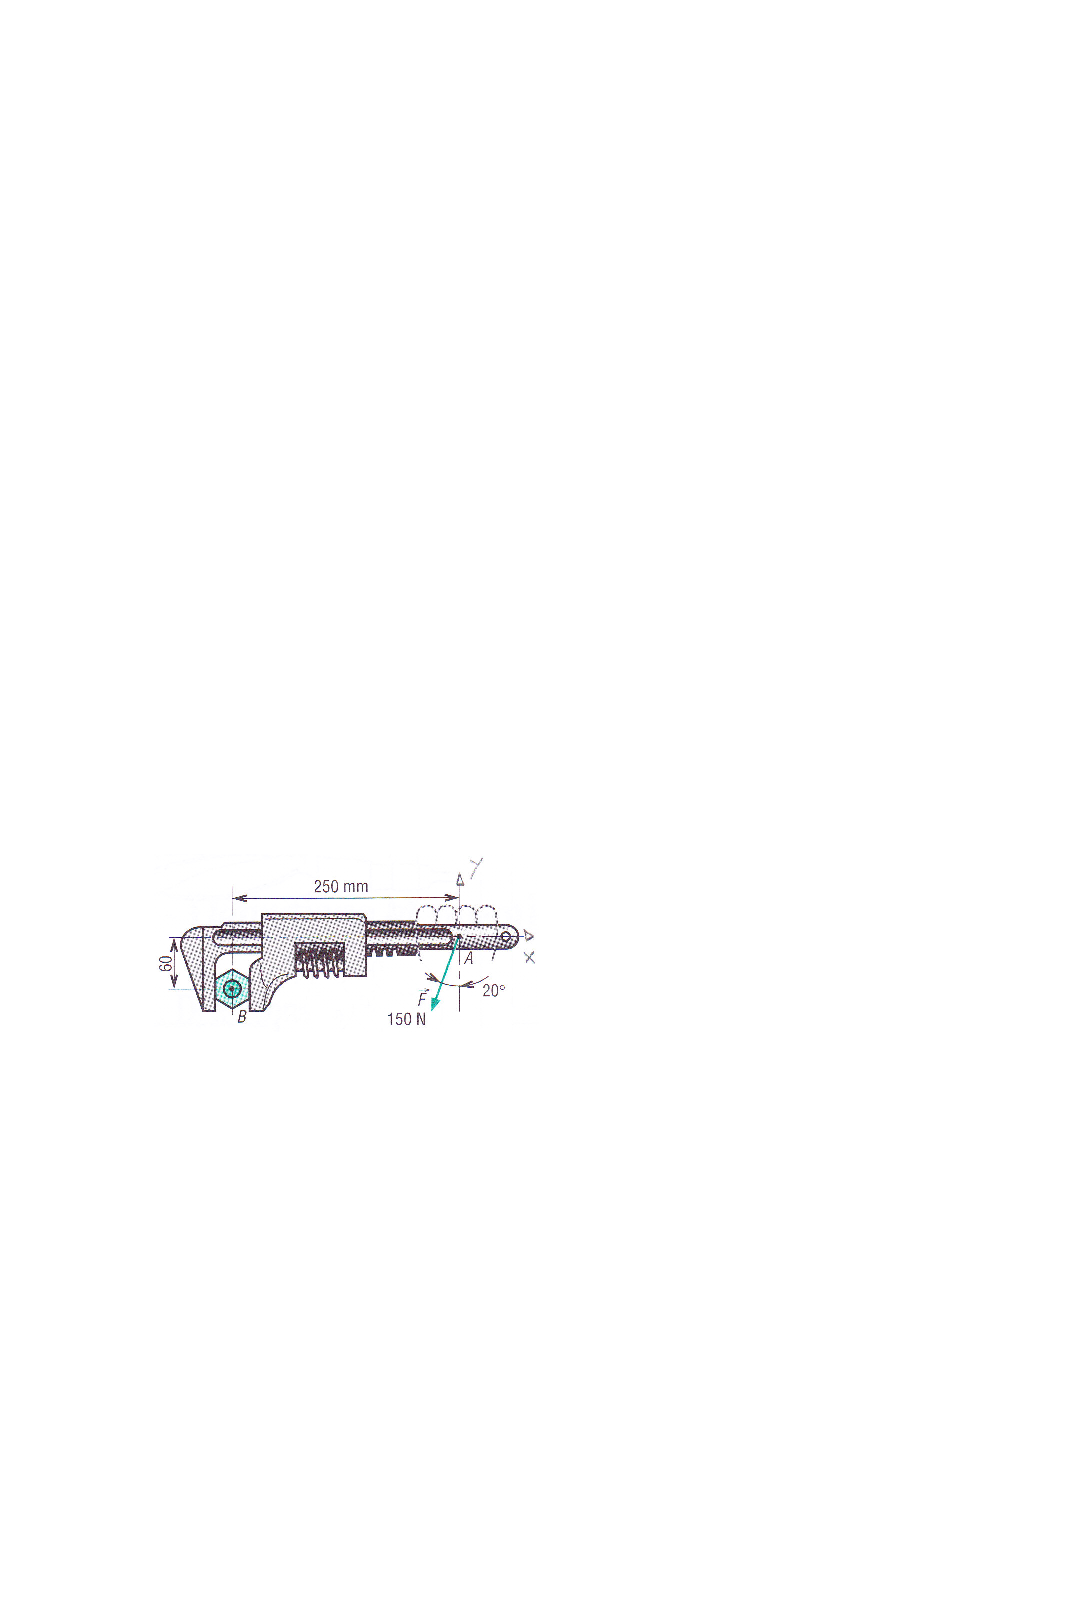
\includegraphics[width=\linewidth]{519_01}
%\caption{Paramétrage de la surface totale et élémentaire en coordonnées sphériques de la demi-voile \label{fig_39_01}}
\end{marginfigure}
\fi

\question{Déterminer $\vect{\mathcal{M}\left(A,\vect{F}\right)}$.}%\vectm{A}{F}{1}{2}$.}
\ifprof ~\\
\else
\fi

\question{Déterminer $\vect{\mathcal{M}\left(B,\vect{F}\right)}$.}%\vectm{A}{F}{1}{2}$.}
\ifprof ~\\
\else
\fi


\ifprof
\else

\marginnote{Corrigé voir \ref{STAT:02:B2:14-gl:519}.}

\fi